% Created by tikzDevice version 0.12.3 on 2020-06-01 10:40:19
% !TEX encoding = UTF-8 Unicode
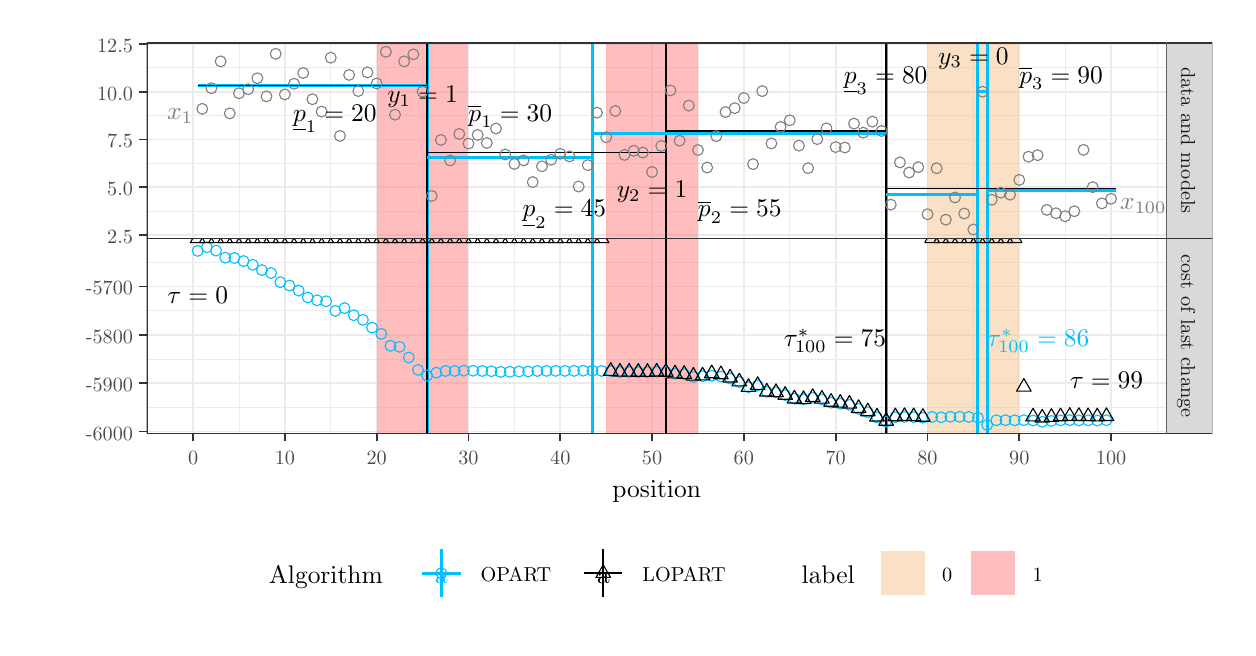
\begin{tikzpicture}[x=1pt,y=1pt]
\definecolor{fillColor}{RGB}{255,255,255}
\path[use as bounding box,fill=fillColor,fill opacity=0.00] (0,0) rectangle (433.62,216.81);
\begin{scope}
\path[clip] (  0.00,  0.00) rectangle (433.62,216.81);
\definecolor{drawColor}{RGB}{255,255,255}
\definecolor{fillColor}{RGB}{255,255,255}

\path[draw=drawColor,line width= 0.6pt,line join=round,line cap=round,fill=fillColor] (  0.00,  0.00) rectangle (433.62,216.81);
\end{scope}
\begin{scope}
\path[clip] ( 43.01,140.67) rectangle (411.55,211.31);
\definecolor{fillColor}{RGB}{255,255,255}

\path[fill=fillColor] ( 43.01,140.67) rectangle (411.55,211.31);
\definecolor{drawColor}{gray}{0.92}

\path[draw=drawColor,line width= 0.3pt,line join=round] ( 43.01,150.50) --
	(411.55,150.50);

\path[draw=drawColor,line width= 0.3pt,line join=round] ( 43.01,167.76) --
	(411.55,167.76);

\path[draw=drawColor,line width= 0.3pt,line join=round] ( 43.01,185.03) --
	(411.55,185.03);

\path[draw=drawColor,line width= 0.3pt,line join=round] ( 43.01,202.29) --
	(411.55,202.29);

\path[draw=drawColor,line width= 0.3pt,line join=round] ( 43.18,140.67) --
	( 43.18,211.31);

\path[draw=drawColor,line width= 0.3pt,line join=round] ( 76.35,140.67) --
	( 76.35,211.31);

\path[draw=drawColor,line width= 0.3pt,line join=round] (109.52,140.67) --
	(109.52,211.31);

\path[draw=drawColor,line width= 0.3pt,line join=round] (142.69,140.67) --
	(142.69,211.31);

\path[draw=drawColor,line width= 0.3pt,line join=round] (175.87,140.67) --
	(175.87,211.31);

\path[draw=drawColor,line width= 0.3pt,line join=round] (209.04,140.67) --
	(209.04,211.31);

\path[draw=drawColor,line width= 0.3pt,line join=round] (242.21,140.67) --
	(242.21,211.31);

\path[draw=drawColor,line width= 0.3pt,line join=round] (275.38,140.67) --
	(275.38,211.31);

\path[draw=drawColor,line width= 0.3pt,line join=round] (308.55,140.67) --
	(308.55,211.31);

\path[draw=drawColor,line width= 0.3pt,line join=round] (341.72,140.67) --
	(341.72,211.31);

\path[draw=drawColor,line width= 0.3pt,line join=round] (374.89,140.67) --
	(374.89,211.31);

\path[draw=drawColor,line width= 0.3pt,line join=round] (408.07,140.67) --
	(408.07,211.31);

\path[draw=drawColor,line width= 0.6pt,line join=round] ( 43.01,141.86) --
	(411.55,141.86);

\path[draw=drawColor,line width= 0.6pt,line join=round] ( 43.01,159.13) --
	(411.55,159.13);

\path[draw=drawColor,line width= 0.6pt,line join=round] ( 43.01,176.39) --
	(411.55,176.39);

\path[draw=drawColor,line width= 0.6pt,line join=round] ( 43.01,193.66) --
	(411.55,193.66);

\path[draw=drawColor,line width= 0.6pt,line join=round] ( 43.01,210.92) --
	(411.55,210.92);

\path[draw=drawColor,line width= 0.6pt,line join=round] ( 59.77,140.67) --
	( 59.77,211.31);

\path[draw=drawColor,line width= 0.6pt,line join=round] ( 92.94,140.67) --
	( 92.94,211.31);

\path[draw=drawColor,line width= 0.6pt,line join=round] (126.11,140.67) --
	(126.11,211.31);

\path[draw=drawColor,line width= 0.6pt,line join=round] (159.28,140.67) --
	(159.28,211.31);

\path[draw=drawColor,line width= 0.6pt,line join=round] (192.45,140.67) --
	(192.45,211.31);

\path[draw=drawColor,line width= 0.6pt,line join=round] (225.62,140.67) --
	(225.62,211.31);

\path[draw=drawColor,line width= 0.6pt,line join=round] (258.79,140.67) --
	(258.79,211.31);

\path[draw=drawColor,line width= 0.6pt,line join=round] (291.97,140.67) --
	(291.97,211.31);

\path[draw=drawColor,line width= 0.6pt,line join=round] (325.14,140.67) --
	(325.14,211.31);

\path[draw=drawColor,line width= 0.6pt,line join=round] (358.31,140.67) --
	(358.31,211.31);

\path[draw=drawColor,line width= 0.6pt,line join=round] (391.48,140.67) --
	(391.48,211.31);
\definecolor{drawColor}{gray}{0.50}

\node[text=drawColor,anchor=base east,inner sep=0pt, outer sep=0pt, scale=  0.92] at ( 59.77,183.66) {$x_{1}$};

\node[text=drawColor,anchor=base west,inner sep=0pt, outer sep=0pt, scale=  0.92] at (394.80,151.18) {$x_{100}$};
\definecolor{fillColor}{RGB}{255,125,125}

\path[fill=fillColor,fill opacity=0.50] (126.11,140.67) rectangle (159.28,211.31);

\path[fill=fillColor,fill opacity=0.50] (209.04,140.67) rectangle (242.21,211.31);
\definecolor{fillColor}{RGB}{246,196,143}

\path[fill=fillColor,fill opacity=0.50] (325.14,140.67) rectangle (358.31,211.31);
\definecolor{drawColor}{RGB}{0,191,255}

\path[draw=drawColor,line width= 1.1pt,line join=round] (144.35,140.67) -- (144.35,211.31);

\path[draw=drawColor,line width= 1.1pt,line join=round] (204.06,140.67) -- (204.06,211.31);

\path[draw=drawColor,line width= 1.1pt,line join=round] (310.21,140.67) -- (310.21,211.31);

\path[draw=drawColor,line width= 1.1pt,line join=round] (343.38,140.67) -- (343.38,211.31);

\path[draw=drawColor,line width= 1.1pt,line join=round] (346.70,140.67) -- (346.70,211.31);
\definecolor{drawColor}{RGB}{0,0,0}

\path[draw=drawColor,line width= 0.6pt,line join=round] (144.35,140.67) -- (144.35,211.31);

\path[draw=drawColor,line width= 0.6pt,line join=round] (230.60,140.67) -- (230.60,211.31);

\path[draw=drawColor,line width= 0.6pt,line join=round] (310.21,140.67) -- (310.21,211.31);
\definecolor{drawColor}{RGB}{0,191,255}

\path[draw=drawColor,line width= 1.1pt,line join=round] ( 61.42,195.97) -- (144.35,195.97);

\path[draw=drawColor,line width= 1.1pt,line join=round] (144.35,170.01) -- (204.06,170.01);

\path[draw=drawColor,line width= 1.1pt,line join=round] (204.06,178.52) -- (310.21,178.52);

\path[draw=drawColor,line width= 1.1pt,line join=round] (310.21,156.37) -- (343.38,156.37);

\path[draw=drawColor,line width= 1.1pt,line join=round] (343.38,193.66) -- (346.70,193.66);

\path[draw=drawColor,line width= 1.1pt,line join=round] (346.70,157.92) -- (393.14,157.92);
\definecolor{drawColor}{RGB}{0,0,0}

\path[draw=drawColor,line width= 0.6pt,line join=round] ( 61.42,195.97) -- (144.35,195.97);

\path[draw=drawColor,line width= 0.6pt,line join=round] (144.35,171.68) -- (230.60,171.68);

\path[draw=drawColor,line width= 0.6pt,line join=round] (230.60,179.54) -- (310.21,179.54);

\path[draw=drawColor,line width= 0.6pt,line join=round] (310.21,158.73) -- (393.14,158.73);
\definecolor{drawColor}{gray}{0.50}

\path[draw=drawColor,line width= 0.4pt,line join=round,line cap=round] ( 63.08,187.47) circle (  1.96);

\path[draw=drawColor,line width= 0.4pt,line join=round,line cap=round] ( 66.40,194.94) circle (  1.96);

\path[draw=drawColor,line width= 0.4pt,line join=round,line cap=round] ( 69.72,204.63) circle (  1.96);

\path[draw=drawColor,line width= 0.4pt,line join=round,line cap=round] ( 73.03,185.85) circle (  1.96);

\path[draw=drawColor,line width= 0.4pt,line join=round,line cap=round] ( 76.35,193.11) circle (  1.96);

\path[draw=drawColor,line width= 0.4pt,line join=round,line cap=round] ( 79.67,194.57) circle (  1.96);

\path[draw=drawColor,line width= 0.4pt,line join=round,line cap=round] ( 82.99,198.55) circle (  1.96);

\path[draw=drawColor,line width= 0.4pt,line join=round,line cap=round] ( 86.30,192.00) circle (  1.96);

\path[draw=drawColor,line width= 0.4pt,line join=round,line cap=round] ( 89.62,207.36) circle (  1.96);

\path[draw=drawColor,line width= 0.4pt,line join=round,line cap=round] ( 92.94,192.70) circle (  1.96);

\path[draw=drawColor,line width= 0.4pt,line join=round,line cap=round] ( 96.25,196.54) circle (  1.96);

\path[draw=drawColor,line width= 0.4pt,line join=round,line cap=round] ( 99.57,200.44) circle (  1.96);

\path[draw=drawColor,line width= 0.4pt,line join=round,line cap=round] (102.89,190.95) circle (  1.96);

\path[draw=drawColor,line width= 0.4pt,line join=round,line cap=round] (106.21,186.48) circle (  1.96);

\path[draw=drawColor,line width= 0.4pt,line join=round,line cap=round] (109.52,205.97) circle (  1.96);

\path[draw=drawColor,line width= 0.4pt,line join=round,line cap=round] (112.84,177.70) circle (  1.96);

\path[draw=drawColor,line width= 0.4pt,line join=round,line cap=round] (116.16,199.73) circle (  1.96);

\path[draw=drawColor,line width= 0.4pt,line join=round,line cap=round] (119.47,193.91) circle (  1.96);

\path[draw=drawColor,line width= 0.4pt,line join=round,line cap=round] (122.79,200.65) circle (  1.96);

\path[draw=drawColor,line width= 0.4pt,line join=round,line cap=round] (126.11,196.64) circle (  1.96);

\path[draw=drawColor,line width= 0.4pt,line join=round,line cap=round] (129.43,208.10) circle (  1.96);

\path[draw=drawColor,line width= 0.4pt,line join=round,line cap=round] (132.74,185.37) circle (  1.96);

\path[draw=drawColor,line width= 0.4pt,line join=round,line cap=round] (136.06,204.64) circle (  1.96);

\path[draw=drawColor,line width= 0.4pt,line join=round,line cap=round] (139.38,207.16) circle (  1.96);

\path[draw=drawColor,line width= 0.4pt,line join=round,line cap=round] (142.69,193.69) circle (  1.96);

\path[draw=drawColor,line width= 0.4pt,line join=round,line cap=round] (146.01,156.01) circle (  1.96);

\path[draw=drawColor,line width= 0.4pt,line join=round,line cap=round] (149.33,176.24) circle (  1.96);

\path[draw=drawColor,line width= 0.4pt,line join=round,line cap=round] (152.65,168.82) circle (  1.96);

\path[draw=drawColor,line width= 0.4pt,line join=round,line cap=round] (155.96,178.41) circle (  1.96);

\path[draw=drawColor,line width= 0.4pt,line join=round,line cap=round] (159.28,174.94) circle (  1.96);

\path[draw=drawColor,line width= 0.4pt,line join=round,line cap=round] (162.60,178.04) circle (  1.96);

\path[draw=drawColor,line width= 0.4pt,line join=round,line cap=round] (165.91,175.14) circle (  1.96);

\path[draw=drawColor,line width= 0.4pt,line join=round,line cap=round] (169.23,180.37) circle (  1.96);

\path[draw=drawColor,line width= 0.4pt,line join=round,line cap=round] (172.55,170.98) circle (  1.96);

\path[draw=drawColor,line width= 0.4pt,line join=round,line cap=round] (175.87,167.58) circle (  1.96);

\path[draw=drawColor,line width= 0.4pt,line join=round,line cap=round] (179.18,168.83) circle (  1.96);

\path[draw=drawColor,line width= 0.4pt,line join=round,line cap=round] (182.50,161.02) circle (  1.96);

\path[draw=drawColor,line width= 0.4pt,line join=round,line cap=round] (185.82,166.71) circle (  1.96);

\path[draw=drawColor,line width= 0.4pt,line join=round,line cap=round] (189.13,169.08) circle (  1.96);

\path[draw=drawColor,line width= 0.4pt,line join=round,line cap=round] (192.45,171.24) circle (  1.96);

\path[draw=drawColor,line width= 0.4pt,line join=round,line cap=round] (195.77,170.29) circle (  1.96);

\path[draw=drawColor,line width= 0.4pt,line join=round,line cap=round] (199.09,159.41) circle (  1.96);

\path[draw=drawColor,line width= 0.4pt,line join=round,line cap=round] (202.40,167.13) circle (  1.96);

\path[draw=drawColor,line width= 0.4pt,line join=round,line cap=round] (205.72,186.09) circle (  1.96);

\path[draw=drawColor,line width= 0.4pt,line join=round,line cap=round] (209.04,177.24) circle (  1.96);

\path[draw=drawColor,line width= 0.4pt,line join=round,line cap=round] (212.35,186.69) circle (  1.96);

\path[draw=drawColor,line width= 0.4pt,line join=round,line cap=round] (215.67,170.83) circle (  1.96);

\path[draw=drawColor,line width= 0.4pt,line join=round,line cap=round] (218.99,172.31) circle (  1.96);

\path[draw=drawColor,line width= 0.4pt,line join=round,line cap=round] (222.31,171.67) circle (  1.96);

\path[draw=drawColor,line width= 0.4pt,line join=round,line cap=round] (225.62,164.66) circle (  1.96);

\path[draw=drawColor,line width= 0.4pt,line join=round,line cap=round] (228.94,174.06) circle (  1.96);

\path[draw=drawColor,line width= 0.4pt,line join=round,line cap=round] (232.26,194.12) circle (  1.96);

\path[draw=drawColor,line width= 0.4pt,line join=round,line cap=round] (235.57,175.96) circle (  1.96);

\path[draw=drawColor,line width= 0.4pt,line join=round,line cap=round] (238.89,188.66) circle (  1.96);

\path[draw=drawColor,line width= 0.4pt,line join=round,line cap=round] (242.21,172.61) circle (  1.96);

\path[draw=drawColor,line width= 0.4pt,line join=round,line cap=round] (245.53,166.27) circle (  1.96);

\path[draw=drawColor,line width= 0.4pt,line join=round,line cap=round] (248.84,177.62) circle (  1.96);

\path[draw=drawColor,line width= 0.4pt,line join=round,line cap=round] (252.16,186.31) circle (  1.96);

\path[draw=drawColor,line width= 0.4pt,line join=round,line cap=round] (255.48,187.72) circle (  1.96);

\path[draw=drawColor,line width= 0.4pt,line join=round,line cap=round] (258.79,191.39) circle (  1.96);

\path[draw=drawColor,line width= 0.4pt,line join=round,line cap=round] (262.11,167.50) circle (  1.96);

\path[draw=drawColor,line width= 0.4pt,line join=round,line cap=round] (265.43,193.88) circle (  1.96);

\path[draw=drawColor,line width= 0.4pt,line join=round,line cap=round] (268.75,174.99) circle (  1.96);

\path[draw=drawColor,line width= 0.4pt,line join=round,line cap=round] (272.06,180.94) circle (  1.96);

\path[draw=drawColor,line width= 0.4pt,line join=round,line cap=round] (275.38,183.34) circle (  1.96);

\path[draw=drawColor,line width= 0.4pt,line join=round,line cap=round] (278.70,174.18) circle (  1.96);

\path[draw=drawColor,line width= 0.4pt,line join=round,line cap=round] (282.01,166.04) circle (  1.96);

\path[draw=drawColor,line width= 0.4pt,line join=round,line cap=round] (285.33,176.54) circle (  1.96);

\path[draw=drawColor,line width= 0.4pt,line join=round,line cap=round] (288.65,180.43) circle (  1.96);

\path[draw=drawColor,line width= 0.4pt,line join=round,line cap=round] (291.97,173.66) circle (  1.96);

\path[draw=drawColor,line width= 0.4pt,line join=round,line cap=round] (295.28,173.49) circle (  1.96);

\path[draw=drawColor,line width= 0.4pt,line join=round,line cap=round] (298.60,182.13) circle (  1.96);

\path[draw=drawColor,line width= 0.4pt,line join=round,line cap=round] (301.92,178.87) circle (  1.96);

\path[draw=drawColor,line width= 0.4pt,line join=round,line cap=round] (305.23,182.85) circle (  1.96);

\path[draw=drawColor,line width= 0.4pt,line join=round,line cap=round] (308.55,179.48) circle (  1.96);

\path[draw=drawColor,line width= 0.4pt,line join=round,line cap=round] (311.87,152.86) circle (  1.96);

\path[draw=drawColor,line width= 0.4pt,line join=round,line cap=round] (315.19,168.13) circle (  1.96);

\path[draw=drawColor,line width= 0.4pt,line join=round,line cap=round] (318.50,164.46) circle (  1.96);

\path[draw=drawColor,line width= 0.4pt,line join=round,line cap=round] (321.82,166.40) circle (  1.96);

\path[draw=drawColor,line width= 0.4pt,line join=round,line cap=round] (325.14,149.39) circle (  1.96);

\path[draw=drawColor,line width= 0.4pt,line join=round,line cap=round] (328.45,166.01) circle (  1.96);

\path[draw=drawColor,line width= 0.4pt,line join=round,line cap=round] (331.77,147.42) circle (  1.96);

\path[draw=drawColor,line width= 0.4pt,line join=round,line cap=round] (335.09,155.45) circle (  1.96);

\path[draw=drawColor,line width= 0.4pt,line join=round,line cap=round] (338.41,149.65) circle (  1.96);

\path[draw=drawColor,line width= 0.4pt,line join=round,line cap=round] (341.72,143.88) circle (  1.96);

\path[draw=drawColor,line width= 0.4pt,line join=round,line cap=round] (345.04,193.66) circle (  1.96);

\path[draw=drawColor,line width= 0.4pt,line join=round,line cap=round] (348.36,154.62) circle (  1.96);

\path[draw=drawColor,line width= 0.4pt,line join=round,line cap=round] (351.67,157.16) circle (  1.96);

\path[draw=drawColor,line width= 0.4pt,line join=round,line cap=round] (354.99,156.46) circle (  1.96);

\path[draw=drawColor,line width= 0.4pt,line join=round,line cap=round] (358.31,161.80) circle (  1.96);

\path[draw=drawColor,line width= 0.4pt,line join=round,line cap=round] (361.63,170.18) circle (  1.96);

\path[draw=drawColor,line width= 0.4pt,line join=round,line cap=round] (364.94,170.74) circle (  1.96);

\path[draw=drawColor,line width= 0.4pt,line join=round,line cap=round] (368.26,150.96) circle (  1.96);

\path[draw=drawColor,line width= 0.4pt,line join=round,line cap=round] (371.58,149.75) circle (  1.96);

\path[draw=drawColor,line width= 0.4pt,line join=round,line cap=round] (374.89,148.68) circle (  1.96);

\path[draw=drawColor,line width= 0.4pt,line join=round,line cap=round] (378.21,150.48) circle (  1.96);

\path[draw=drawColor,line width= 0.4pt,line join=round,line cap=round] (381.53,172.66) circle (  1.96);

\path[draw=drawColor,line width= 0.4pt,line join=round,line cap=round] (384.85,159.18) circle (  1.96);

\path[draw=drawColor,line width= 0.4pt,line join=round,line cap=round] (388.16,153.31) circle (  1.96);

\path[draw=drawColor,line width= 0.4pt,line join=round,line cap=round] (391.48,154.98) circle (  1.96);
\definecolor{drawColor}{RGB}{0,0,0}

\node[text=drawColor,anchor=base east,inner sep=0pt, outer sep=0pt, scale=  0.92] at (126.11,182.95) {$\underline p_{1}=20$};

\node[text=drawColor,anchor=base east,inner sep=0pt, outer sep=0pt, scale=  0.92] at (209.04,148.42) {$\underline p_{2}=45$};

\node[text=drawColor,anchor=base east,inner sep=0pt, outer sep=0pt, scale=  0.92] at (325.14,196.76) {$\underline p_{3}=80$};

\node[text=drawColor,anchor=base,inner sep=0pt, outer sep=0pt, scale=  0.92] at (142.69,189.86) {$y_{1}=1$};

\node[text=drawColor,anchor=base,inner sep=0pt, outer sep=0pt, scale=  0.92] at (225.62,155.33) {$y_{2}=1$};

\node[text=drawColor,anchor=base,inner sep=0pt, outer sep=0pt, scale=  0.92] at (341.72,203.67) {$y_{3}=0$};

\node[text=drawColor,anchor=base west,inner sep=0pt, outer sep=0pt, scale=  0.92] at (159.28,182.95) {$\overline p_{1}=30$};

\node[text=drawColor,anchor=base west,inner sep=0pt, outer sep=0pt, scale=  0.92] at (242.21,148.42) {$\overline p_{2}=55$};

\node[text=drawColor,anchor=base west,inner sep=0pt, outer sep=0pt, scale=  0.92] at (358.31,196.76) {$\overline p_{3}=90$};
\definecolor{drawColor}{gray}{0.20}

\path[draw=drawColor,line width= 0.6pt,line join=round,line cap=round] ( 43.01,140.67) rectangle (411.55,211.31);
\end{scope}
\begin{scope}
\path[clip] ( 43.01, 70.03) rectangle (411.55,140.67);
\definecolor{fillColor}{RGB}{255,255,255}

\path[fill=fillColor] ( 43.01, 70.03) rectangle (411.55,140.67);
\definecolor{drawColor}{gray}{0.92}

\path[draw=drawColor,line width= 0.3pt,line join=round] ( 43.01, 79.59) --
	(411.55, 79.59);

\path[draw=drawColor,line width= 0.3pt,line join=round] ( 43.01, 97.08) --
	(411.55, 97.08);

\path[draw=drawColor,line width= 0.3pt,line join=round] ( 43.01,114.58) --
	(411.55,114.58);

\path[draw=drawColor,line width= 0.3pt,line join=round] ( 43.01,132.07) --
	(411.55,132.07);

\path[draw=drawColor,line width= 0.3pt,line join=round] ( 43.18, 70.03) --
	( 43.18,140.67);

\path[draw=drawColor,line width= 0.3pt,line join=round] ( 76.35, 70.03) --
	( 76.35,140.67);

\path[draw=drawColor,line width= 0.3pt,line join=round] (109.52, 70.03) --
	(109.52,140.67);

\path[draw=drawColor,line width= 0.3pt,line join=round] (142.69, 70.03) --
	(142.69,140.67);

\path[draw=drawColor,line width= 0.3pt,line join=round] (175.87, 70.03) --
	(175.87,140.67);

\path[draw=drawColor,line width= 0.3pt,line join=round] (209.04, 70.03) --
	(209.04,140.67);

\path[draw=drawColor,line width= 0.3pt,line join=round] (242.21, 70.03) --
	(242.21,140.67);

\path[draw=drawColor,line width= 0.3pt,line join=round] (275.38, 70.03) --
	(275.38,140.67);

\path[draw=drawColor,line width= 0.3pt,line join=round] (308.55, 70.03) --
	(308.55,140.67);

\path[draw=drawColor,line width= 0.3pt,line join=round] (341.72, 70.03) --
	(341.72,140.67);

\path[draw=drawColor,line width= 0.3pt,line join=round] (374.89, 70.03) --
	(374.89,140.67);

\path[draw=drawColor,line width= 0.3pt,line join=round] (408.07, 70.03) --
	(408.07,140.67);

\path[draw=drawColor,line width= 0.6pt,line join=round] ( 43.01, 70.84) --
	(411.55, 70.84);

\path[draw=drawColor,line width= 0.6pt,line join=round] ( 43.01, 88.34) --
	(411.55, 88.34);

\path[draw=drawColor,line width= 0.6pt,line join=round] ( 43.01,105.83) --
	(411.55,105.83);

\path[draw=drawColor,line width= 0.6pt,line join=round] ( 43.01,123.33) --
	(411.55,123.33);

\path[draw=drawColor,line width= 0.6pt,line join=round] ( 59.77, 70.03) --
	( 59.77,140.67);

\path[draw=drawColor,line width= 0.6pt,line join=round] ( 92.94, 70.03) --
	( 92.94,140.67);

\path[draw=drawColor,line width= 0.6pt,line join=round] (126.11, 70.03) --
	(126.11,140.67);

\path[draw=drawColor,line width= 0.6pt,line join=round] (159.28, 70.03) --
	(159.28,140.67);

\path[draw=drawColor,line width= 0.6pt,line join=round] (192.45, 70.03) --
	(192.45,140.67);

\path[draw=drawColor,line width= 0.6pt,line join=round] (225.62, 70.03) --
	(225.62,140.67);

\path[draw=drawColor,line width= 0.6pt,line join=round] (258.79, 70.03) --
	(258.79,140.67);

\path[draw=drawColor,line width= 0.6pt,line join=round] (291.97, 70.03) --
	(291.97,140.67);

\path[draw=drawColor,line width= 0.6pt,line join=round] (325.14, 70.03) --
	(325.14,140.67);

\path[draw=drawColor,line width= 0.6pt,line join=round] (358.31, 70.03) --
	(358.31,140.67);

\path[draw=drawColor,line width= 0.6pt,line join=round] (391.48, 70.03) --
	(391.48,140.67);
\definecolor{fillColor}{RGB}{255,125,125}

\path[fill=fillColor,fill opacity=0.50] (126.11, 70.03) rectangle (159.28,140.67);

\path[fill=fillColor,fill opacity=0.50] (209.04, 70.03) rectangle (242.21,140.67);
\definecolor{fillColor}{RGB}{246,196,143}

\path[fill=fillColor,fill opacity=0.50] (325.14, 70.03) rectangle (358.31,140.67);
\definecolor{drawColor}{RGB}{0,191,255}

\path[draw=drawColor,line width= 1.1pt,line join=round] (144.35, 70.03) -- (144.35,140.67);

\path[draw=drawColor,line width= 1.1pt,line join=round] (204.06, 70.03) -- (204.06,140.67);

\path[draw=drawColor,line width= 1.1pt,line join=round] (310.21, 70.03) -- (310.21,140.67);

\path[draw=drawColor,line width= 1.1pt,line join=round] (343.38, 70.03) -- (343.38,140.67);

\path[draw=drawColor,line width= 1.1pt,line join=round] (346.70, 70.03) -- (346.70,140.67);
\definecolor{drawColor}{RGB}{0,0,0}

\path[draw=drawColor,line width= 0.6pt,line join=round] (144.35, 70.03) -- (144.35,140.67);

\path[draw=drawColor,line width= 0.6pt,line join=round] (230.60, 70.03) -- (230.60,140.67);

\path[draw=drawColor,line width= 0.6pt,line join=round] (310.21, 70.03) -- (310.21,140.67);

\node[text=drawColor,anchor=base,inner sep=0pt, outer sep=0pt, scale=  0.92] at ( 61.42,117.15) {$\tau = 0$};

\node[text=drawColor,anchor=base,inner sep=0pt, outer sep=0pt, scale=  0.92] at (389.82, 86.36) {$\tau = 99$};
\definecolor{drawColor}{RGB}{0,191,255}

\node[text=drawColor,anchor=base west,inner sep=0pt, outer sep=0pt, scale=  0.92] at (346.70,101.55) {$\tau^*_{100} = 86$};
\definecolor{drawColor}{RGB}{0,0,0}

\node[text=drawColor,anchor=base east,inner sep=0pt, outer sep=0pt, scale=  0.92] at (310.21,101.55) {$\tau^*_{100} = 75$};
\definecolor{drawColor}{RGB}{0,191,255}

\path[draw=drawColor,line width= 0.4pt,line join=round,line cap=round] ( 61.42,136.16) circle (  1.96);

\path[draw=drawColor,line width= 0.4pt,line join=round,line cap=round] ( 64.74,137.46) circle (  1.96);

\path[draw=drawColor,line width= 0.4pt,line join=round,line cap=round] ( 68.06,136.27) circle (  1.96);

\path[draw=drawColor,line width= 0.4pt,line join=round,line cap=round] ( 71.38,133.70) circle (  1.96);

\path[draw=drawColor,line width= 0.4pt,line join=round,line cap=round] ( 74.69,133.59) circle (  1.96);

\path[draw=drawColor,line width= 0.4pt,line join=round,line cap=round] ( 78.01,132.47) circle (  1.96);

\path[draw=drawColor,line width= 0.4pt,line join=round,line cap=round] ( 81.33,131.13) circle (  1.96);

\path[draw=drawColor,line width= 0.4pt,line join=round,line cap=round] ( 84.64,129.21) circle (  1.96);

\path[draw=drawColor,line width= 0.4pt,line join=round,line cap=round] ( 87.96,128.16) circle (  1.96);

\path[draw=drawColor,line width= 0.4pt,line join=round,line cap=round] ( 91.28,124.84) circle (  1.96);

\path[draw=drawColor,line width= 0.4pt,line join=round,line cap=round] ( 94.60,123.64) circle (  1.96);

\path[draw=drawColor,line width= 0.4pt,line join=round,line cap=round] ( 97.91,121.81) circle (  1.96);

\path[draw=drawColor,line width= 0.4pt,line join=round,line cap=round] (101.23,119.32) circle (  1.96);

\path[draw=drawColor,line width= 0.4pt,line join=round,line cap=round] (104.55,118.30) circle (  1.96);

\path[draw=drawColor,line width= 0.4pt,line join=round,line cap=round] (107.86,117.95) circle (  1.96);

\path[draw=drawColor,line width= 0.4pt,line join=round,line cap=round] (111.18,114.46) circle (  1.96);

\path[draw=drawColor,line width= 0.4pt,line join=round,line cap=round] (114.50,115.46) circle (  1.96);

\path[draw=drawColor,line width= 0.4pt,line join=round,line cap=round] (117.82,112.91) circle (  1.96);

\path[draw=drawColor,line width= 0.4pt,line join=round,line cap=round] (121.13,111.23) circle (  1.96);

\path[draw=drawColor,line width= 0.4pt,line join=round,line cap=round] (124.45,108.40) circle (  1.96);

\path[draw=drawColor,line width= 0.4pt,line join=round,line cap=round] (127.77,106.16) circle (  1.96);

\path[draw=drawColor,line width= 0.4pt,line join=round,line cap=round] (131.08,101.85) circle (  1.96);

\path[draw=drawColor,line width= 0.4pt,line join=round,line cap=round] (134.40,101.48) circle (  1.96);

\path[draw=drawColor,line width= 0.4pt,line join=round,line cap=round] (137.72, 97.62) circle (  1.96);

\path[draw=drawColor,line width= 0.4pt,line join=round,line cap=round] (141.04, 93.15) circle (  1.96);

\path[draw=drawColor,line width= 0.4pt,line join=round,line cap=round] (144.35, 91.11) circle (  1.96);

\path[draw=drawColor,line width= 0.4pt,line join=round,line cap=round] (147.67, 92.15) circle (  1.96);

\path[draw=drawColor,line width= 0.4pt,line join=round,line cap=round] (150.99, 92.76) circle (  1.96);

\path[draw=drawColor,line width= 0.4pt,line join=round,line cap=round] (154.30, 92.77) circle (  1.96);

\path[draw=drawColor,line width= 0.4pt,line join=round,line cap=round] (157.62, 92.86) circle (  1.96);

\path[draw=drawColor,line width= 0.4pt,line join=round,line cap=round] (160.94, 92.84) circle (  1.96);

\path[draw=drawColor,line width= 0.4pt,line join=round,line cap=round] (164.26, 92.75) circle (  1.96);

\path[draw=drawColor,line width= 0.4pt,line join=round,line cap=round] (167.57, 92.67) circle (  1.96);

\path[draw=drawColor,line width= 0.4pt,line join=round,line cap=round] (170.89, 92.43) circle (  1.96);

\path[draw=drawColor,line width= 0.4pt,line join=round,line cap=round] (174.21, 92.45) circle (  1.96);

\path[draw=drawColor,line width= 0.4pt,line join=round,line cap=round] (177.52, 92.54) circle (  1.96);

\path[draw=drawColor,line width= 0.4pt,line join=round,line cap=round] (180.84, 92.58) circle (  1.96);

\path[draw=drawColor,line width= 0.4pt,line join=round,line cap=round] (184.16, 92.75) circle (  1.96);

\path[draw=drawColor,line width= 0.4pt,line join=round,line cap=round] (187.48, 92.79) circle (  1.96);

\path[draw=drawColor,line width= 0.4pt,line join=round,line cap=round] (190.79, 92.80) circle (  1.96);

\path[draw=drawColor,line width= 0.4pt,line join=round,line cap=round] (194.11, 92.79) circle (  1.96);

\path[draw=drawColor,line width= 0.4pt,line join=round,line cap=round] (197.43, 92.79) circle (  1.96);

\path[draw=drawColor,line width= 0.4pt,line join=round,line cap=round] (200.74, 92.86) circle (  1.96);

\path[draw=drawColor,line width= 0.4pt,line join=round,line cap=round] (204.06, 92.86) circle (  1.96);

\path[draw=drawColor,line width= 0.4pt,line join=round,line cap=round] (207.38, 92.77) circle (  1.96);

\path[draw=drawColor,line width= 0.4pt,line join=round,line cap=round] (210.70, 92.69) circle (  1.96);

\path[draw=drawColor,line width= 0.4pt,line join=round,line cap=round] (214.01, 92.42) circle (  1.96);

\path[draw=drawColor,line width= 0.4pt,line join=round,line cap=round] (217.33, 92.41) circle (  1.96);

\path[draw=drawColor,line width= 0.4pt,line join=round,line cap=round] (220.65, 92.37) circle (  1.96);

\path[draw=drawColor,line width= 0.4pt,line join=round,line cap=round] (223.96, 92.35) circle (  1.96);

\path[draw=drawColor,line width= 0.4pt,line join=round,line cap=round] (227.28, 92.46) circle (  1.96);

\path[draw=drawColor,line width= 0.4pt,line join=round,line cap=round] (230.60, 92.39) circle (  1.96);

\path[draw=drawColor,line width= 0.4pt,line join=round,line cap=round] (233.92, 91.76) circle (  1.96);

\path[draw=drawColor,line width= 0.4pt,line join=round,line cap=round] (237.23, 91.62) circle (  1.96);

\path[draw=drawColor,line width= 0.4pt,line join=round,line cap=round] (240.55, 90.62) circle (  1.96);

\path[draw=drawColor,line width= 0.4pt,line join=round,line cap=round] (243.87, 90.88) circle (  1.96);

\path[draw=drawColor,line width= 0.4pt,line join=round,line cap=round] (247.18, 91.04) circle (  1.96);

\path[draw=drawColor,line width= 0.4pt,line join=round,line cap=round] (250.50, 90.75) circle (  1.96);

\path[draw=drawColor,line width= 0.4pt,line join=round,line cap=round] (253.82, 90.03) circle (  1.96);

\path[draw=drawColor,line width= 0.4pt,line join=round,line cap=round] (257.14, 88.77) circle (  1.96);

\path[draw=drawColor,line width= 0.4pt,line join=round,line cap=round] (260.45, 86.91) circle (  1.96);

\path[draw=drawColor,line width= 0.4pt,line join=round,line cap=round] (263.77, 87.49) circle (  1.96);

\path[draw=drawColor,line width= 0.4pt,line join=round,line cap=round] (267.09, 85.24) circle (  1.96);

\path[draw=drawColor,line width= 0.4pt,line join=round,line cap=round] (270.40, 85.04) circle (  1.96);

\path[draw=drawColor,line width= 0.4pt,line join=round,line cap=round] (273.72, 84.06) circle (  1.96);

\path[draw=drawColor,line width= 0.4pt,line join=round,line cap=round] (277.04, 82.73) circle (  1.96);

\path[draw=drawColor,line width= 0.4pt,line join=round,line cap=round] (280.36, 82.51) circle (  1.96);

\path[draw=drawColor,line width= 0.4pt,line join=round,line cap=round] (283.67, 83.08) circle (  1.96);

\path[draw=drawColor,line width= 0.4pt,line join=round,line cap=round] (286.99, 82.46) circle (  1.96);

\path[draw=drawColor,line width= 0.4pt,line join=round,line cap=round] (290.31, 81.33) circle (  1.96);

\path[draw=drawColor,line width= 0.4pt,line join=round,line cap=round] (293.62, 80.95) circle (  1.96);

\path[draw=drawColor,line width= 0.4pt,line join=round,line cap=round] (296.94, 80.54) circle (  1.96);

\path[draw=drawColor,line width= 0.4pt,line join=round,line cap=round] (300.26, 79.03) circle (  1.96);

\path[draw=drawColor,line width= 0.4pt,line join=round,line cap=round] (303.58, 77.82) circle (  1.96);

\path[draw=drawColor,line width= 0.4pt,line join=round,line cap=round] (306.89, 75.97) circle (  1.96);

\path[draw=drawColor,line width= 0.4pt,line join=round,line cap=round] (310.21, 74.46) circle (  1.96);

\path[draw=drawColor,line width= 0.4pt,line join=round,line cap=round] (313.53, 76.07) circle (  1.96);

\path[draw=drawColor,line width= 0.4pt,line join=round,line cap=round] (316.84, 76.18) circle (  1.96);

\path[draw=drawColor,line width= 0.4pt,line join=round,line cap=round] (320.16, 76.09) circle (  1.96);

\path[draw=drawColor,line width= 0.4pt,line join=round,line cap=round] (323.48, 75.89) circle (  1.96);

\path[draw=drawColor,line width= 0.4pt,line join=round,line cap=round] (326.80, 76.15) circle (  1.96);

\path[draw=drawColor,line width= 0.4pt,line join=round,line cap=round] (330.11, 76.03) circle (  1.96);

\path[draw=drawColor,line width= 0.4pt,line join=round,line cap=round] (333.43, 76.20) circle (  1.96);

\path[draw=drawColor,line width= 0.4pt,line join=round,line cap=round] (336.75, 76.21) circle (  1.96);

\path[draw=drawColor,line width= 0.4pt,line join=round,line cap=round] (340.06, 76.16) circle (  1.96);

\path[draw=drawColor,line width= 0.4pt,line join=round,line cap=round] (343.38, 75.86) circle (  1.96);

\path[draw=drawColor,line width= 0.4pt,line join=round,line cap=round] (346.70, 73.24) circle (  1.96);

\path[draw=drawColor,line width= 0.4pt,line join=round,line cap=round] (350.02, 74.95) circle (  1.96);

\path[draw=drawColor,line width= 0.4pt,line join=round,line cap=round] (353.33, 74.96) circle (  1.96);

\path[draw=drawColor,line width= 0.4pt,line join=round,line cap=round] (356.65, 74.94) circle (  1.96);

\path[draw=drawColor,line width= 0.4pt,line join=round,line cap=round] (359.97, 74.99) circle (  1.96);

\path[draw=drawColor,line width= 0.4pt,line join=round,line cap=round] (363.28, 74.86) circle (  1.96);

\path[draw=drawColor,line width= 0.4pt,line join=round,line cap=round] (366.60, 74.40) circle (  1.96);

\path[draw=drawColor,line width= 0.4pt,line join=round,line cap=round] (369.92, 74.71) circle (  1.96);

\path[draw=drawColor,line width= 0.4pt,line join=round,line cap=round] (373.24, 74.92) circle (  1.96);

\path[draw=drawColor,line width= 0.4pt,line join=round,line cap=round] (376.55, 74.99) circle (  1.96);

\path[draw=drawColor,line width= 0.4pt,line join=round,line cap=round] (379.87, 74.90) circle (  1.96);

\path[draw=drawColor,line width= 0.4pt,line join=round,line cap=round] (383.19, 74.93) circle (  1.96);

\path[draw=drawColor,line width= 0.4pt,line join=round,line cap=round] (386.50, 74.87) circle (  1.96);

\path[draw=drawColor,line width= 0.4pt,line join=round,line cap=round] (389.82, 74.96) circle (  1.96);
\definecolor{drawColor}{RGB}{0,0,0}

\path[draw=drawColor,line width= 0.4pt,line join=round,line cap=round] ( 61.42,143.72) --
	( 64.07,139.14) --
	( 58.78,139.14) --
	( 61.42,143.72);

\path[draw=drawColor,line width= 0.4pt,line join=round,line cap=round] ( 64.74,143.72) --
	( 67.38,139.14) --
	( 62.10,139.14) --
	( 64.74,143.72);

\path[draw=drawColor,line width= 0.4pt,line join=round,line cap=round] ( 68.06,143.72) --
	( 70.70,139.14) --
	( 65.42,139.14) --
	( 68.06,143.72);

\path[draw=drawColor,line width= 0.4pt,line join=round,line cap=round] ( 71.38,143.72) --
	( 74.02,139.14) --
	( 68.73,139.14) --
	( 71.38,143.72);

\path[draw=drawColor,line width= 0.4pt,line join=round,line cap=round] ( 74.69,143.72) --
	( 77.34,139.14) --
	( 72.05,139.14) --
	( 74.69,143.72);

\path[draw=drawColor,line width= 0.4pt,line join=round,line cap=round] ( 78.01,143.72) --
	( 80.65,139.14) --
	( 75.37,139.14) --
	( 78.01,143.72);

\path[draw=drawColor,line width= 0.4pt,line join=round,line cap=round] ( 81.33,143.72) --
	( 83.97,139.14) --
	( 78.68,139.14) --
	( 81.33,143.72);

\path[draw=drawColor,line width= 0.4pt,line join=round,line cap=round] ( 84.64,143.72) --
	( 87.29,139.14) --
	( 82.00,139.14) --
	( 84.64,143.72);

\path[draw=drawColor,line width= 0.4pt,line join=round,line cap=round] ( 87.96,143.72) --
	( 90.60,139.14) --
	( 85.32,139.14) --
	( 87.96,143.72);

\path[draw=drawColor,line width= 0.4pt,line join=round,line cap=round] ( 91.28,143.72) --
	( 93.92,139.14) --
	( 88.64,139.14) --
	( 91.28,143.72);

\path[draw=drawColor,line width= 0.4pt,line join=round,line cap=round] ( 94.60,143.72) --
	( 97.24,139.14) --
	( 91.95,139.14) --
	( 94.60,143.72);

\path[draw=drawColor,line width= 0.4pt,line join=round,line cap=round] ( 97.91,143.72) --
	(100.56,139.14) --
	( 95.27,139.14) --
	( 97.91,143.72);

\path[draw=drawColor,line width= 0.4pt,line join=round,line cap=round] (101.23,143.72) --
	(103.87,139.14) --
	( 98.59,139.14) --
	(101.23,143.72);

\path[draw=drawColor,line width= 0.4pt,line join=round,line cap=round] (104.55,143.72) --
	(107.19,139.14) --
	(101.90,139.14) --
	(104.55,143.72);

\path[draw=drawColor,line width= 0.4pt,line join=round,line cap=round] (107.86,143.72) --
	(110.51,139.14) --
	(105.22,139.14) --
	(107.86,143.72);

\path[draw=drawColor,line width= 0.4pt,line join=round,line cap=round] (111.18,143.72) --
	(113.82,139.14) --
	(108.54,139.14) --
	(111.18,143.72);

\path[draw=drawColor,line width= 0.4pt,line join=round,line cap=round] (114.50,143.72) --
	(117.14,139.14) --
	(111.86,139.14) --
	(114.50,143.72);

\path[draw=drawColor,line width= 0.4pt,line join=round,line cap=round] (117.82,143.72) --
	(120.46,139.14) --
	(115.17,139.14) --
	(117.82,143.72);

\path[draw=drawColor,line width= 0.4pt,line join=round,line cap=round] (121.13,143.72) --
	(123.78,139.14) --
	(118.49,139.14) --
	(121.13,143.72);

\path[draw=drawColor,line width= 0.4pt,line join=round,line cap=round] (124.45,143.72) --
	(127.09,139.14) --
	(121.81,139.14) --
	(124.45,143.72);

\path[draw=drawColor,line width= 0.4pt,line join=round,line cap=round] (127.77,143.72) --
	(130.41,139.14) --
	(125.12,139.14) --
	(127.77,143.72);

\path[draw=drawColor,line width= 0.4pt,line join=round,line cap=round] (131.08,143.72) --
	(133.73,139.14) --
	(128.44,139.14) --
	(131.08,143.72);

\path[draw=drawColor,line width= 0.4pt,line join=round,line cap=round] (134.40,143.72) --
	(137.04,139.14) --
	(131.76,139.14) --
	(134.40,143.72);

\path[draw=drawColor,line width= 0.4pt,line join=round,line cap=round] (137.72,143.72) --
	(140.36,139.14) --
	(135.08,139.14) --
	(137.72,143.72);

\path[draw=drawColor,line width= 0.4pt,line join=round,line cap=round] (141.04,143.72) --
	(143.68,139.14) --
	(138.39,139.14) --
	(141.04,143.72);

\path[draw=drawColor,line width= 0.4pt,line join=round,line cap=round] (144.35,143.72) --
	(147.00,139.14) --
	(141.71,139.14) --
	(144.35,143.72);

\path[draw=drawColor,line width= 0.4pt,line join=round,line cap=round] (147.67,143.72) --
	(150.31,139.14) --
	(145.03,139.14) --
	(147.67,143.72);

\path[draw=drawColor,line width= 0.4pt,line join=round,line cap=round] (150.99,143.72) --
	(153.63,139.14) --
	(148.34,139.14) --
	(150.99,143.72);

\path[draw=drawColor,line width= 0.4pt,line join=round,line cap=round] (154.30,143.72) --
	(156.95,139.14) --
	(151.66,139.14) --
	(154.30,143.72);

\path[draw=drawColor,line width= 0.4pt,line join=round,line cap=round] (157.62,143.72) --
	(160.26,139.14) --
	(154.98,139.14) --
	(157.62,143.72);

\path[draw=drawColor,line width= 0.4pt,line join=round,line cap=round] (160.94,143.72) --
	(163.58,139.14) --
	(158.30,139.14) --
	(160.94,143.72);

\path[draw=drawColor,line width= 0.4pt,line join=round,line cap=round] (164.26,143.72) --
	(166.90,139.14) --
	(161.61,139.14) --
	(164.26,143.72);

\path[draw=drawColor,line width= 0.4pt,line join=round,line cap=round] (167.57,143.72) --
	(170.22,139.14) --
	(164.93,139.14) --
	(167.57,143.72);

\path[draw=drawColor,line width= 0.4pt,line join=round,line cap=round] (170.89,143.72) --
	(173.53,139.14) --
	(168.25,139.14) --
	(170.89,143.72);

\path[draw=drawColor,line width= 0.4pt,line join=round,line cap=round] (174.21,143.72) --
	(176.85,139.14) --
	(171.56,139.14) --
	(174.21,143.72);

\path[draw=drawColor,line width= 0.4pt,line join=round,line cap=round] (177.52,143.72) --
	(180.17,139.14) --
	(174.88,139.14) --
	(177.52,143.72);

\path[draw=drawColor,line width= 0.4pt,line join=round,line cap=round] (180.84,143.72) --
	(183.48,139.14) --
	(178.20,139.14) --
	(180.84,143.72);

\path[draw=drawColor,line width= 0.4pt,line join=round,line cap=round] (184.16,143.72) --
	(186.80,139.14) --
	(181.52,139.14) --
	(184.16,143.72);

\path[draw=drawColor,line width= 0.4pt,line join=round,line cap=round] (187.48,143.72) --
	(190.12,139.14) --
	(184.83,139.14) --
	(187.48,143.72);

\path[draw=drawColor,line width= 0.4pt,line join=round,line cap=round] (190.79,143.72) --
	(193.44,139.14) --
	(188.15,139.14) --
	(190.79,143.72);

\path[draw=drawColor,line width= 0.4pt,line join=round,line cap=round] (194.11,143.72) --
	(196.75,139.14) --
	(191.47,139.14) --
	(194.11,143.72);

\path[draw=drawColor,line width= 0.4pt,line join=round,line cap=round] (197.43,143.72) --
	(200.07,139.14) --
	(194.78,139.14) --
	(197.43,143.72);

\path[draw=drawColor,line width= 0.4pt,line join=round,line cap=round] (200.74,143.72) --
	(203.39,139.14) --
	(198.10,139.14) --
	(200.74,143.72);

\path[draw=drawColor,line width= 0.4pt,line join=round,line cap=round] (204.06,143.72) --
	(206.70,139.14) --
	(201.42,139.14) --
	(204.06,143.72);

\path[draw=drawColor,line width= 0.4pt,line join=round,line cap=round] (207.38,143.72) --
	(210.02,139.14) --
	(204.74,139.14) --
	(207.38,143.72);

\path[draw=drawColor,line width= 0.4pt,line join=round,line cap=round] (210.70, 95.75) --
	(213.34, 91.17) --
	(208.05, 91.17) --
	(210.70, 95.75);

\path[draw=drawColor,line width= 0.4pt,line join=round,line cap=round] (214.01, 95.47) --
	(216.66, 90.89) --
	(211.37, 90.89) --
	(214.01, 95.47);

\path[draw=drawColor,line width= 0.4pt,line join=round,line cap=round] (217.33, 95.46) --
	(219.97, 90.89) --
	(214.69, 90.89) --
	(217.33, 95.46);

\path[draw=drawColor,line width= 0.4pt,line join=round,line cap=round] (220.65, 95.42) --
	(223.29, 90.85) --
	(218.00, 90.85) --
	(220.65, 95.42);

\path[draw=drawColor,line width= 0.4pt,line join=round,line cap=round] (223.96, 95.40) --
	(226.61, 90.82) --
	(221.32, 90.82) --
	(223.96, 95.40);

\path[draw=drawColor,line width= 0.4pt,line join=round,line cap=round] (227.28, 95.51) --
	(229.92, 90.94) --
	(224.64, 90.94) --
	(227.28, 95.51);

\path[draw=drawColor,line width= 0.4pt,line join=round,line cap=round] (230.60, 95.44) --
	(233.24, 90.86) --
	(227.96, 90.86) --
	(230.60, 95.44);

\path[draw=drawColor,line width= 0.4pt,line join=round,line cap=round] (233.92, 94.84) --
	(236.56, 90.26) --
	(231.27, 90.26) --
	(233.92, 94.84);

\path[draw=drawColor,line width= 0.4pt,line join=round,line cap=round] (237.23, 94.67) --
	(239.88, 90.09) --
	(234.59, 90.09) --
	(237.23, 94.67);

\path[draw=drawColor,line width= 0.4pt,line join=round,line cap=round] (240.55, 94.01) --
	(243.19, 89.43) --
	(237.91, 89.43) --
	(240.55, 94.01);

\path[draw=drawColor,line width= 0.4pt,line join=round,line cap=round] (243.87, 94.10) --
	(246.51, 89.52) --
	(241.22, 89.52) --
	(243.87, 94.10);

\path[draw=drawColor,line width= 0.4pt,line join=round,line cap=round] (247.18, 94.89) --
	(249.83, 90.32) --
	(244.54, 90.32) --
	(247.18, 94.89);

\path[draw=drawColor,line width= 0.4pt,line join=round,line cap=round] (250.50, 94.54) --
	(253.14, 89.96) --
	(247.86, 89.96) --
	(250.50, 94.54);

\path[draw=drawColor,line width= 0.4pt,line join=round,line cap=round] (253.82, 93.36) --
	(256.46, 88.79) --
	(251.18, 88.79) --
	(253.82, 93.36);

\path[draw=drawColor,line width= 0.4pt,line join=round,line cap=round] (257.14, 91.94) --
	(259.78, 87.36) --
	(254.49, 87.36) --
	(257.14, 91.94);

\path[draw=drawColor,line width= 0.4pt,line join=round,line cap=round] (260.45, 89.96) --
	(263.10, 85.38) --
	(257.81, 85.38) --
	(260.45, 89.96);

\path[draw=drawColor,line width= 0.4pt,line join=round,line cap=round] (263.77, 90.67) --
	(266.41, 86.09) --
	(261.13, 86.09) --
	(263.77, 90.67);

\path[draw=drawColor,line width= 0.4pt,line join=round,line cap=round] (267.09, 88.29) --
	(269.73, 83.71) --
	(264.44, 83.71) --
	(267.09, 88.29);

\path[draw=drawColor,line width= 0.4pt,line join=round,line cap=round] (270.40, 88.09) --
	(273.05, 83.51) --
	(267.76, 83.51) --
	(270.40, 88.09);

\path[draw=drawColor,line width= 0.4pt,line join=round,line cap=round] (273.72, 87.11) --
	(276.36, 82.54) --
	(271.08, 82.54) --
	(273.72, 87.11);

\path[draw=drawColor,line width= 0.4pt,line join=round,line cap=round] (277.04, 85.78) --
	(279.68, 81.20) --
	(274.40, 81.20) --
	(277.04, 85.78);

\path[draw=drawColor,line width= 0.4pt,line join=round,line cap=round] (280.36, 85.56) --
	(283.00, 80.98) --
	(277.71, 80.98) --
	(280.36, 85.56);

\path[draw=drawColor,line width= 0.4pt,line join=round,line cap=round] (283.67, 86.31) --
	(286.32, 81.73) --
	(281.03, 81.73) --
	(283.67, 86.31);

\path[draw=drawColor,line width= 0.4pt,line join=round,line cap=round] (286.99, 85.71) --
	(289.63, 81.13) --
	(284.35, 81.13) --
	(286.99, 85.71);

\path[draw=drawColor,line width= 0.4pt,line join=round,line cap=round] (290.31, 84.58) --
	(292.95, 80.00) --
	(287.66, 80.00) --
	(290.31, 84.58);

\path[draw=drawColor,line width= 0.4pt,line join=round,line cap=round] (293.62, 84.24) --
	(296.27, 79.67) --
	(290.98, 79.67) --
	(293.62, 84.24);

\path[draw=drawColor,line width= 0.4pt,line join=round,line cap=round] (296.94, 83.89) --
	(299.58, 79.31) --
	(294.30, 79.31) --
	(296.94, 83.89);

\path[draw=drawColor,line width= 0.4pt,line join=round,line cap=round] (300.26, 82.34) --
	(302.90, 77.76) --
	(297.62, 77.76) --
	(300.26, 82.34);

\path[draw=drawColor,line width= 0.4pt,line join=round,line cap=round] (303.58, 81.13) --
	(306.22, 76.56) --
	(300.93, 76.56) --
	(303.58, 81.13);

\path[draw=drawColor,line width= 0.4pt,line join=round,line cap=round] (306.89, 79.26) --
	(309.54, 74.68) --
	(304.25, 74.68) --
	(306.89, 79.26);

\path[draw=drawColor,line width= 0.4pt,line join=round,line cap=round] (310.21, 77.74) --
	(312.85, 73.16) --
	(307.57, 73.16) --
	(310.21, 77.74);

\path[draw=drawColor,line width= 0.4pt,line join=round,line cap=round] (313.53, 79.36) --
	(316.17, 74.78) --
	(310.88, 74.78) --
	(313.53, 79.36);

\path[draw=drawColor,line width= 0.4pt,line join=round,line cap=round] (316.84, 79.46) --
	(319.49, 74.89) --
	(314.20, 74.89) --
	(316.84, 79.46);

\path[draw=drawColor,line width= 0.4pt,line join=round,line cap=round] (320.16, 79.37) --
	(322.80, 74.79) --
	(317.52, 74.79) --
	(320.16, 79.37);

\path[draw=drawColor,line width= 0.4pt,line join=round,line cap=round] (323.48, 79.17) --
	(326.12, 74.60) --
	(320.84, 74.60) --
	(323.48, 79.17);

\path[draw=drawColor,line width= 0.4pt,line join=round,line cap=round] (326.80,143.72) --
	(329.44,139.14) --
	(324.15,139.14) --
	(326.80,143.72);

\path[draw=drawColor,line width= 0.4pt,line join=round,line cap=round] (330.11,143.72) --
	(332.76,139.14) --
	(327.47,139.14) --
	(330.11,143.72);

\path[draw=drawColor,line width= 0.4pt,line join=round,line cap=round] (333.43,143.72) --
	(336.07,139.14) --
	(330.79,139.14) --
	(333.43,143.72);

\path[draw=drawColor,line width= 0.4pt,line join=round,line cap=round] (336.75,143.72) --
	(339.39,139.14) --
	(334.10,139.14) --
	(336.75,143.72);

\path[draw=drawColor,line width= 0.4pt,line join=round,line cap=round] (340.06,143.72) --
	(342.71,139.14) --
	(337.42,139.14) --
	(340.06,143.72);

\path[draw=drawColor,line width= 0.4pt,line join=round,line cap=round] (343.38,143.72) --
	(346.02,139.14) --
	(340.74,139.14) --
	(343.38,143.72);

\path[draw=drawColor,line width= 0.4pt,line join=round,line cap=round] (346.70,143.72) --
	(349.34,139.14) --
	(344.06,139.14) --
	(346.70,143.72);

\path[draw=drawColor,line width= 0.4pt,line join=round,line cap=round] (350.02,143.72) --
	(352.66,139.14) --
	(347.37,139.14) --
	(350.02,143.72);

\path[draw=drawColor,line width= 0.4pt,line join=round,line cap=round] (353.33,143.72) --
	(355.98,139.14) --
	(350.69,139.14) --
	(353.33,143.72);

\path[draw=drawColor,line width= 0.4pt,line join=round,line cap=round] (356.65,143.72) --
	(359.29,139.14) --
	(354.01,139.14) --
	(356.65,143.72);

\path[draw=drawColor,line width= 0.4pt,line join=round,line cap=round] (359.97, 90.03) --
	(362.61, 85.46) --
	(357.32, 85.46) --
	(359.97, 90.03);

\path[draw=drawColor,line width= 0.4pt,line join=round,line cap=round] (363.28, 79.28) --
	(365.93, 74.71) --
	(360.64, 74.71) --
	(363.28, 79.28);

\path[draw=drawColor,line width= 0.4pt,line join=round,line cap=round] (366.60, 78.89) --
	(369.24, 74.31) --
	(363.96, 74.31) --
	(366.60, 78.89);

\path[draw=drawColor,line width= 0.4pt,line join=round,line cap=round] (369.92, 79.13) --
	(372.56, 74.56) --
	(367.28, 74.56) --
	(369.92, 79.13);

\path[draw=drawColor,line width= 0.4pt,line join=round,line cap=round] (373.24, 79.35) --
	(375.88, 74.77) --
	(370.59, 74.77) --
	(373.24, 79.35);

\path[draw=drawColor,line width= 0.4pt,line join=round,line cap=round] (376.55, 79.48) --
	(379.20, 74.90) --
	(373.91, 74.90) --
	(376.55, 79.48);

\path[draw=drawColor,line width= 0.4pt,line join=round,line cap=round] (379.87, 79.46) --
	(382.51, 74.88) --
	(377.23, 74.88) --
	(379.87, 79.46);

\path[draw=drawColor,line width= 0.4pt,line join=round,line cap=round] (383.19, 79.38) --
	(385.83, 74.80) --
	(380.54, 74.80) --
	(383.19, 79.38);

\path[draw=drawColor,line width= 0.4pt,line join=round,line cap=round] (386.50, 79.32) --
	(389.15, 74.74) --
	(383.86, 74.74) --
	(386.50, 79.32);

\path[draw=drawColor,line width= 0.4pt,line join=round,line cap=round] (389.82, 79.43) --
	(392.46, 74.86) --
	(387.18, 74.86) --
	(389.82, 79.43);
\definecolor{drawColor}{gray}{0.20}

\path[draw=drawColor,line width= 0.6pt,line join=round,line cap=round] ( 43.01, 70.03) rectangle (411.55,140.67);
\end{scope}
\begin{scope}
\path[clip] (411.55,140.67) rectangle (428.12,211.31);
\definecolor{drawColor}{gray}{0.20}
\definecolor{fillColor}{gray}{0.85}

\path[draw=drawColor,line width= 0.6pt,line join=round,line cap=round,fill=fillColor] (411.55,140.67) rectangle (428.12,211.31);
\definecolor{drawColor}{gray}{0.10}

\node[text=drawColor,rotate=-90.00,anchor=base,inner sep=0pt, outer sep=0pt, scale=  0.73] at (416.80,175.99) {data and models};
\end{scope}
\begin{scope}
\path[clip] (411.55, 70.03) rectangle (428.12,140.67);
\definecolor{drawColor}{gray}{0.20}
\definecolor{fillColor}{gray}{0.85}

\path[draw=drawColor,line width= 0.6pt,line join=round,line cap=round,fill=fillColor] (411.55, 70.03) rectangle (428.12,140.67);
\definecolor{drawColor}{gray}{0.10}

\node[text=drawColor,rotate=-90.00,anchor=base,inner sep=0pt, outer sep=0pt, scale=  0.73] at (416.80,105.35) {cost of last change};
\end{scope}
\begin{scope}
\path[clip] (  0.00,  0.00) rectangle (433.62,216.81);
\definecolor{drawColor}{gray}{0.20}

\path[draw=drawColor,line width= 0.6pt,line join=round] ( 59.77, 67.28) --
	( 59.77, 70.03);

\path[draw=drawColor,line width= 0.6pt,line join=round] ( 92.94, 67.28) --
	( 92.94, 70.03);

\path[draw=drawColor,line width= 0.6pt,line join=round] (126.11, 67.28) --
	(126.11, 70.03);

\path[draw=drawColor,line width= 0.6pt,line join=round] (159.28, 67.28) --
	(159.28, 70.03);

\path[draw=drawColor,line width= 0.6pt,line join=round] (192.45, 67.28) --
	(192.45, 70.03);

\path[draw=drawColor,line width= 0.6pt,line join=round] (225.62, 67.28) --
	(225.62, 70.03);

\path[draw=drawColor,line width= 0.6pt,line join=round] (258.79, 67.28) --
	(258.79, 70.03);

\path[draw=drawColor,line width= 0.6pt,line join=round] (291.97, 67.28) --
	(291.97, 70.03);

\path[draw=drawColor,line width= 0.6pt,line join=round] (325.14, 67.28) --
	(325.14, 70.03);

\path[draw=drawColor,line width= 0.6pt,line join=round] (358.31, 67.28) --
	(358.31, 70.03);

\path[draw=drawColor,line width= 0.6pt,line join=round] (391.48, 67.28) --
	(391.48, 70.03);
\end{scope}
\begin{scope}
\path[clip] (  0.00,  0.00) rectangle (433.62,216.81);
\definecolor{drawColor}{gray}{0.30}

\node[text=drawColor,anchor=base,inner sep=0pt, outer sep=0pt, scale=  0.73] at ( 59.77, 59.02) {0};

\node[text=drawColor,anchor=base,inner sep=0pt, outer sep=0pt, scale=  0.73] at ( 92.94, 59.02) {10};

\node[text=drawColor,anchor=base,inner sep=0pt, outer sep=0pt, scale=  0.73] at (126.11, 59.02) {20};

\node[text=drawColor,anchor=base,inner sep=0pt, outer sep=0pt, scale=  0.73] at (159.28, 59.02) {30};

\node[text=drawColor,anchor=base,inner sep=0pt, outer sep=0pt, scale=  0.73] at (192.45, 59.02) {40};

\node[text=drawColor,anchor=base,inner sep=0pt, outer sep=0pt, scale=  0.73] at (225.62, 59.02) {50};

\node[text=drawColor,anchor=base,inner sep=0pt, outer sep=0pt, scale=  0.73] at (258.79, 59.02) {60};

\node[text=drawColor,anchor=base,inner sep=0pt, outer sep=0pt, scale=  0.73] at (291.97, 59.02) {70};

\node[text=drawColor,anchor=base,inner sep=0pt, outer sep=0pt, scale=  0.73] at (325.14, 59.02) {80};

\node[text=drawColor,anchor=base,inner sep=0pt, outer sep=0pt, scale=  0.73] at (358.31, 59.02) {90};

\node[text=drawColor,anchor=base,inner sep=0pt, outer sep=0pt, scale=  0.73] at (391.48, 59.02) {100};
\end{scope}
\begin{scope}
\path[clip] (  0.00,  0.00) rectangle (433.62,216.81);
\definecolor{drawColor}{gray}{0.30}

\node[text=drawColor,anchor=base east,inner sep=0pt, outer sep=0pt, scale=  0.73] at ( 38.06,138.83) {2.5};

\node[text=drawColor,anchor=base east,inner sep=0pt, outer sep=0pt, scale=  0.73] at ( 38.06,156.10) {5.0};

\node[text=drawColor,anchor=base east,inner sep=0pt, outer sep=0pt, scale=  0.73] at ( 38.06,173.36) {7.5};

\node[text=drawColor,anchor=base east,inner sep=0pt, outer sep=0pt, scale=  0.73] at ( 38.06,190.63) {10.0};

\node[text=drawColor,anchor=base east,inner sep=0pt, outer sep=0pt, scale=  0.73] at ( 38.06,207.89) {12.5};
\end{scope}
\begin{scope}
\path[clip] (  0.00,  0.00) rectangle (433.62,216.81);
\definecolor{drawColor}{gray}{0.20}

\path[draw=drawColor,line width= 0.6pt,line join=round] ( 40.26,141.86) --
	( 43.01,141.86);

\path[draw=drawColor,line width= 0.6pt,line join=round] ( 40.26,159.13) --
	( 43.01,159.13);

\path[draw=drawColor,line width= 0.6pt,line join=round] ( 40.26,176.39) --
	( 43.01,176.39);

\path[draw=drawColor,line width= 0.6pt,line join=round] ( 40.26,193.66) --
	( 43.01,193.66);

\path[draw=drawColor,line width= 0.6pt,line join=round] ( 40.26,210.92) --
	( 43.01,210.92);
\end{scope}
\begin{scope}
\path[clip] (  0.00,  0.00) rectangle (433.62,216.81);
\definecolor{drawColor}{gray}{0.30}

\node[text=drawColor,anchor=base east,inner sep=0pt, outer sep=0pt, scale=  0.73] at ( 38.06, 67.81) {-6000};

\node[text=drawColor,anchor=base east,inner sep=0pt, outer sep=0pt, scale=  0.73] at ( 38.06, 85.31) {-5900};

\node[text=drawColor,anchor=base east,inner sep=0pt, outer sep=0pt, scale=  0.73] at ( 38.06,102.80) {-5800};

\node[text=drawColor,anchor=base east,inner sep=0pt, outer sep=0pt, scale=  0.73] at ( 38.06,120.30) {-5700};
\end{scope}
\begin{scope}
\path[clip] (  0.00,  0.00) rectangle (433.62,216.81);
\definecolor{drawColor}{gray}{0.20}

\path[draw=drawColor,line width= 0.6pt,line join=round] ( 40.26, 70.84) --
	( 43.01, 70.84);

\path[draw=drawColor,line width= 0.6pt,line join=round] ( 40.26, 88.34) --
	( 43.01, 88.34);

\path[draw=drawColor,line width= 0.6pt,line join=round] ( 40.26,105.83) --
	( 43.01,105.83);

\path[draw=drawColor,line width= 0.6pt,line join=round] ( 40.26,123.33) --
	( 43.01,123.33);
\end{scope}
\begin{scope}
\path[clip] (  0.00,  0.00) rectangle (433.62,216.81);
\definecolor{drawColor}{RGB}{0,0,0}

\node[text=drawColor,anchor=base,inner sep=0pt, outer sep=0pt, scale=  0.92] at (227.28, 46.98) {position};
\end{scope}
\begin{scope}
\path[clip] (  0.00,  0.00) rectangle (433.62,216.81);
\definecolor{fillColor}{RGB}{255,255,255}

\path[fill=fillColor] ( 81.65,  5.50) rectangle (263.17, 33.84);
\end{scope}
\begin{scope}
\path[clip] (  0.00,  0.00) rectangle (433.62,216.81);
\definecolor{drawColor}{RGB}{0,0,0}

\node[text=drawColor,anchor=base west,inner sep=0pt, outer sep=0pt, scale=  0.92] at ( 87.15, 15.88) {Algorithm};
\end{scope}
\begin{scope}
\path[clip] (  0.00,  0.00) rectangle (433.62,216.81);
\definecolor{fillColor}{RGB}{255,255,255}

\path[fill=fillColor] (140.81, 11.00) rectangle (158.16, 28.34);
\end{scope}
\begin{scope}
\path[clip] (  0.00,  0.00) rectangle (433.62,216.81);
\definecolor{drawColor}{RGB}{0,191,255}

\path[draw=drawColor,line width= 1.1pt,line join=round] (149.48, 11.00) -- (149.48, 28.34);
\end{scope}
\begin{scope}
\path[clip] (  0.00,  0.00) rectangle (433.62,216.81);
\definecolor{drawColor}{RGB}{0,191,255}

\path[draw=drawColor,line width= 1.1pt,line join=round] (142.55, 19.67) -- (156.42, 19.67);
\end{scope}
\begin{scope}
\path[clip] (  0.00,  0.00) rectangle (433.62,216.81);
\definecolor{drawColor}{RGB}{0,191,255}

\node[text=drawColor,anchor=base,inner sep=0pt, outer sep=0pt, scale=  0.92] at (149.48, 15.87) {a};
\end{scope}
\begin{scope}
\path[clip] (  0.00,  0.00) rectangle (433.62,216.81);
\definecolor{drawColor}{RGB}{0,191,255}

\path[draw=drawColor,line width= 0.4pt,line join=round,line cap=round] (149.48, 19.67) circle (  1.96);
\end{scope}
\begin{scope}
\path[clip] (  0.00,  0.00) rectangle (433.62,216.81);
\definecolor{fillColor}{RGB}{255,255,255}

\path[fill=fillColor] (199.30, 11.00) rectangle (216.64, 28.34);
\end{scope}
\begin{scope}
\path[clip] (  0.00,  0.00) rectangle (433.62,216.81);
\definecolor{drawColor}{RGB}{0,0,0}

\path[draw=drawColor,line width= 0.6pt,line join=round] (207.97, 11.00) -- (207.97, 28.34);
\end{scope}
\begin{scope}
\path[clip] (  0.00,  0.00) rectangle (433.62,216.81);
\definecolor{drawColor}{RGB}{0,0,0}

\path[draw=drawColor,line width= 0.6pt,line join=round] (201.03, 19.67) -- (214.91, 19.67);
\end{scope}
\begin{scope}
\path[clip] (  0.00,  0.00) rectangle (433.62,216.81);
\definecolor{drawColor}{RGB}{0,0,0}

\node[text=drawColor,anchor=base,inner sep=0pt, outer sep=0pt, scale=  0.92] at (207.97, 15.87) {a};
\end{scope}
\begin{scope}
\path[clip] (  0.00,  0.00) rectangle (433.62,216.81);
\definecolor{drawColor}{RGB}{0,0,0}

\path[draw=drawColor,line width= 0.4pt,line join=round,line cap=round] (207.97, 22.72) --
	(210.61, 18.15) --
	(205.33, 18.15) --
	(207.97, 22.72);
\end{scope}
\begin{scope}
\path[clip] (  0.00,  0.00) rectangle (433.62,216.81);
\definecolor{drawColor}{RGB}{0,0,0}

\node[text=drawColor,anchor=base west,inner sep=0pt, outer sep=0pt, scale=  0.73] at (163.66, 16.64) {OPART};
\end{scope}
\begin{scope}
\path[clip] (  0.00,  0.00) rectangle (433.62,216.81);
\definecolor{drawColor}{RGB}{0,0,0}

\node[text=drawColor,anchor=base west,inner sep=0pt, outer sep=0pt, scale=  0.73] at (222.14, 16.64) {LOPART};
\end{scope}
\begin{scope}
\path[clip] (  0.00,  0.00) rectangle (433.62,216.81);
\definecolor{fillColor}{RGB}{255,255,255}

\path[fill=fillColor] (274.17,  5.50) rectangle (372.91, 33.84);
\end{scope}
\begin{scope}
\path[clip] (  0.00,  0.00) rectangle (433.62,216.81);
\definecolor{drawColor}{RGB}{0,0,0}

\node[text=drawColor,anchor=base west,inner sep=0pt, outer sep=0pt, scale=  0.92] at (279.67, 15.88) {label};
\end{scope}
\begin{scope}
\path[clip] (  0.00,  0.00) rectangle (433.62,216.81);
\definecolor{fillColor}{RGB}{255,255,255}

\path[fill=fillColor] (307.60, 11.00) rectangle (324.95, 28.34);
\end{scope}
\begin{scope}
\path[clip] (  0.00,  0.00) rectangle (433.62,216.81);
\definecolor{fillColor}{RGB}{246,196,143}

\path[fill=fillColor,fill opacity=0.50] (308.32, 11.71) rectangle (324.24, 27.63);
\end{scope}
\begin{scope}
\path[clip] (  0.00,  0.00) rectangle (433.62,216.81);
\definecolor{fillColor}{RGB}{255,255,255}

\path[fill=fillColor] (340.26, 11.00) rectangle (357.60, 28.34);
\end{scope}
\begin{scope}
\path[clip] (  0.00,  0.00) rectangle (433.62,216.81);
\definecolor{fillColor}{RGB}{255,125,125}

\path[fill=fillColor,fill opacity=0.50] (340.97, 11.71) rectangle (356.89, 27.63);
\end{scope}
\begin{scope}
\path[clip] (  0.00,  0.00) rectangle (433.62,216.81);
\definecolor{drawColor}{RGB}{0,0,0}

\node[text=drawColor,anchor=base west,inner sep=0pt, outer sep=0pt, scale=  0.73] at (330.45, 16.64) {0};
\end{scope}
\begin{scope}
\path[clip] (  0.00,  0.00) rectangle (433.62,216.81);
\definecolor{drawColor}{RGB}{0,0,0}

\node[text=drawColor,anchor=base west,inner sep=0pt, outer sep=0pt, scale=  0.73] at (363.10, 16.64) {1};
\end{scope}
\end{tikzpicture}
